% Created 2021-05-13 Thu 15:44
% Intended LaTeX compiler: pdflatex
\documentclass[a4paper]{article}
\usepackage[utf8]{inputenc}
\usepackage[T1]{fontenc}
\usepackage{graphicx}
\usepackage{grffile}
\usepackage{longtable}
\usepackage{wrapfig}
\usepackage{rotating}
\usepackage[normalem]{ulem}
\usepackage{amsmath}
\usepackage{textcomp}
\usepackage{amssymb}
\usepackage{capt-of}
\usepackage{hyperref}
\input{baseHeader.tex}
\titel{\textbf{Bachelorproject}} \undertitel{Cryptographic library for FPGA's} \opgave{Bachelor Project} \forfatter{Jacob Herbst(mwr148), Jonas Flach Jensen (sjm233)} \dato{12 june 2021} \vejleder{Advisor: Kenneth Skovhede}
\date{}
\title{}
\begin{document}

\maketitle
\tableofcontents
\newpage
\section{Introduction}
\label{sec:org19dae89}

\section{Background}
\label{sec:orga037939}

\subsection{Field Programmable Gate Arrays}
\label{sec:org081eee0}
TODO: write something more in-depth.
Fields Programmable Gate Arrays (FPGA's) is an integrated circuit which can be reconfigured in the ``field''. It stands as the opposite Application Specific Integrated Circuit, which will have the single purpose, whereas FPGA's can be reprogrammed to have different purposes. It means an FPGA can be configured to work as a CPU, a GPU or something else entirely. This is done in hardware description language and typically run through a program to sythesize the design on the FPGA.
FPGA's consist of a set of Configurable Logic Gates (CLBs) and interconnects between these. CLBs is the reason FPGA's is reprogrammable. They differs from classic logic gates such as Nand, etc. used CPU in that they are constructed by look up tables, which can be reprogrammed, instead of gates which are fixed. Since these lookup tables can be build for specific purposes FPGAs can be a programmed to do one thing and do it really well. This lack of generality is often good for both performance and power consumption, compared to a CPU which needs to be able to do general prosessing, and thus in general has a lot of waste.

\subsection{Synchronous Message Exchange}
\label{SME}
Synchronous Message Exchange (SME) is a programming model to enable FPGA development using high-level languages. SME is based on Communicating Sequential Processes (CSP) and at its core constructs from said process calculi, making use of the elements which has proven useful in hardware design\cite{sme}. Using the following concepts from the CSP model\cite{CSP}, SME can be derived:

\begin{itemize}
\item A program consists of a set of named processes.
\item Each process runs on its own processor with no form of sharing with other processes.
\item Concurrent processes can communicate using message passing.
\end{itemize}

SME has a similar notion of processes. There exist two types of SME processes, \texttt{simple process} and a \texttt{simulation process}. Of these, the simple process corresponds to a process in CSP as described above. Each simple process in SME will only share communication channels and constants with the other processes. Simple processes will consist of a set of input and output busses, a \texttt{onTick} function which will run on every clock tick and a set of optional variables and functions. Since the model revolves around mapping to hardware every construct inside a simple process should have a static size. Meaning no dynamic lists, while-loops etc. Simulation processes on the otherhand will not be a part of the actual hardware design, hereby making dynamic constructs legal.
For the communications channels, SME extends the concepts from CSP by using buses. Instead of using explicit naming for sources and destinations, each process will consist of a set of input and output busses that it can read and write to, respectively. Furthermore, these buses use broadcasting as means of synchronization instead of the blocking non-buffered approach.  The broadcasting happens every clock-cycle on the internal clock.
A bus is essentially just a collection of fields that can be read and written to depending on the process' access, merely a data transfer object. Thus a simple (and pointless) process that adds two numbers might have two input busses X\{valid,x\} and Y\{valid,y\}. inside the \texttt{onTick} function, which will be run every tick of the internal clock of SME, could then add the two values x and y if their valid fields was set to true and write the result to a bus RES\{valid, res\}. It is worth noting that a process should not necessarily have one and possibly multiple ``valid''-flags which shows if there is any data on the bus, but this is common in cases where the processes communicate using the ready/valid handshake for instance the one specified by the AXI protocols\footnote{AXI ref}, which is the process communications protocol we wil be using. It is easy to see how an SME model can be transformed into a dependency graph with processes being nodes and buses the edges.From the dependency graph it is possible to create an AST which can be translated into VHDL code\cite{SME}, thus creating the bridge from the high level model to the low-level hardware implementation. This in turn can be fed into a tool such as Xilinx vivado to synthesize the implementation to actual hardware. For the cryptographic library covered in this report we will be using a C\# implementation of SME by the models creators\cite{SME}.
\subsection{A crypto library}
\label{sec:org1815be4}
Cryptographic functions are used by developers across most branches, whether it'll be communicating securely over a network, or hashing programs to do version control.
So there is a motive for having a crypto library for FPGA's. In fact, such a processor has been made before. IBM created their own ``IBM 4758 Secure Coprocessor''\cite{IBM4758}. Another point is modern Hardware Security Modules (HSM) which also does this.
However, the problem with the existing solutions is that many of them require setting up a royalty-based licensing deal, which makes it difficult to use for experimental development, small projects, and in research, and academics.
So we set out to create an open-source crypto library.

The crypto library consists of an implementation of various cryptographic functions, such as AES and SHA256. It should also have an API allowing users to utilize these functions in their projects, as they would with any other library.
These implementations should also be optimized in terms of speed so that they are competitive with the existing software solutions.
Creating a crypto library for FPGA's \ldots{}
\subsubsection{Hashing}
\label{sec:org70c6b53}
Hashing is a mathematical concept referring to using a hash function to map some data of arbitrary size to a value of a fixed size. Cryptographic hash functions are a subset of all hash functions.
The reason for this is that for a hash function to be a cryptographic hash function it needs to uphold several properties to ensure it is secure, such as ensuring that it is hard to find collisions. Computers also have limited space in memory which limits the implementation of hash functions. Lastly and most importantly, computers can't do true randomness.
If a hash function can be implemented with a limited input space, is pseudo-random, and upholds certain properties listed below, it can be categorized as a ``Cryptographic Hash Function''. One such example is the outdated MD5 algorithm.
\begin{itemize}
\item It should be deterministic, as it is important that the same hash is computed given some input.
\item It is unreasonably hard to predict the hashed value. One reason for this is the requirement to exercise the avalanche effect, meaning the tiniest change in the input message would resolve in big changes in the hash.
\item It is collision-resistant, meaning it is unreasonably hard to find two distinct messages to have the same hash.
\end{itemize}

\begin{enumerate}
\item Merkle-Damgård construction
\label{sec:org663afbc}
One approach that is widely used in cryptographic hashing is the Merkle-Damgård construction. One of the reasons this approach is desirable when developing a cryptographic hashing algorithm is because the hash function will be collision-resistant given the compression function itself is collision-resistant.
From Figure \ref{fig:Merkle} one can see the construction of the hashing function. One can see that the message will be padded to have a certain length since any compression function must work on static size. The compression function \texttt{f} will initially take two arguments, the initialization vector, and the first block. f will then produce a result of the same size as the initialization vector. This result will then be fed into the next iteration of \texttt{f} along with the second block of the message. This is repeated until the entire padded message has been processed. From here a potential finalization function can be used to improve the hash. Lastly, the hashed value will be produced.

\begin{figure}[htbp]
\centering
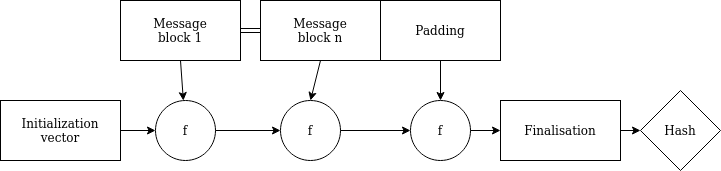
\includegraphics[width=.9\linewidth]{Background/merkle.png}
\caption{\label{fig:Merkle}Merkle-Damgård construction}
\end{figure}
\end{enumerate}
\subsubsection{Cypher}
\label{sec:org6b927f3}
TODO: WRITE SOMETHING ABOUT CYPHERS

\subsection{MD5}
\label{MD5alg}
The Message-Digest algorithm MD5 is a reasonably simple one-way hashing function that produces a 128-bit digest specified in 1992 in RFC 1321\cite{rfc1321}.
THe MD5 algorithm will  thus create a the 128-bit digest from a arbitrary sized message of n bits. Since MD5 uses a merkel damgaard construction, it follows figure\ref{fig:merkel}. It will thus partition the n bit message into smaller blocks of 512 bits. This is done by following a fairly common padding scheme, seen in the merkel damgaard family. It is done by always padding the message with a single set bit followed by a series of 0's until the message length = 448 mod 512. Thus in situations where the original message has a length of 448 mod 512, a 1 is followed by 511 bits of 0's. Lastly, a merkel damgaard strengthening is applied by appending a 64-bit representation of the message length mod 2\textsuperscript{64} to the padded message, resulting in every partiotion being 512 bits wide.
Each partition of the message will then be fed into the compression \texttt{f} function in Figure \ref{fig:merkel}.

\begin{figure}[htbp]
\centering
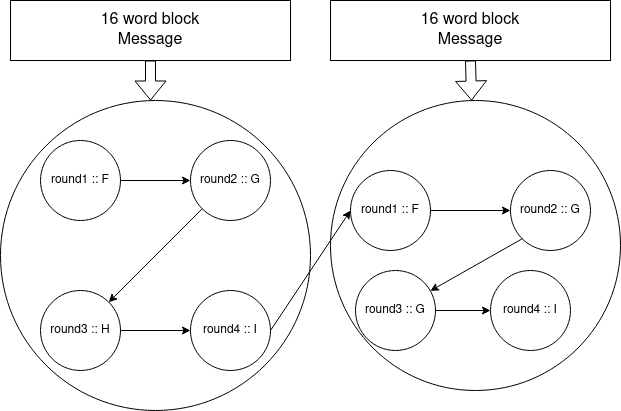
\includegraphics[width=.9\linewidth]{./Background/MD5rounds.png}
\caption{\label{fig:MD5}Two iterations of the MD5 rounds.}
\end{figure}

Figure \ref{fig:MD5} shows the expanded compression function \texttt{f}. \texttt{f} will modify a 128-bit initialization vector (A, B, C, D), with the initial value:\\
\texttt{[} \texttt{A: 0x67542301}, \texttt{B: 0xefcdab89}, \texttt{C: 0x98badcfe}, \texttt{D: 0x10325476} \texttt{]}\\
\texttt{f} will use the following 4 functions, defined as such to, in ``bitwise parallel'' produce independent and unbiased bits in each of the rounds.
\begin{equation}
F(X, Y, Z) = (X \wedge Y) \vee (\neg X \wedge Z) \\
G(X, Y, Z) = (X \wedge Z) \vee (Y \wedge \neg Z) \\
H(X, Y, Z) = X \oplus Y \oplus Z \\
I(X, Y, Z) = Y \oplus ( X \vee \neg Z) \\
\end{equation}
In \texttt{f} a total number of 64 rounds will be computed, each of the functions 1-4 is applied a total of 16 times. Figure \ref{fig:MD5Rounds} shows each of the specific rounds, where \texttt{[abcd k s i]} denotes \texttt{a = b + (( a + round(b,c,d) + M[k] + K[i]) \textbackslash{}lll s)}, where \texttt{round} denotes the function corresponding to one of the 4 functions corresponding to that round, \texttt{M} denotes the current 16-word buffer of the padded message and \texttt{K[i]} denotes the \texttt{floor(2\textasciicircum{}32 * abs (sin(i + 1)))}.
\begin{verbatim}
round 1  :: F
[ABCD  0  7  1] [DABC  1 12  2] [CDAB  2 17  3] [BCDA  3 22  4]
[ABCD  4  7  5] [DABC  5 12  6] [CDAB  6 17  7] [BCDA  7 22  8]
[ABCD  8  7  9] [DABC  9 12 10] [CDAB 10 17 11] [BCDA 11 22 12]
[ABCD 12  7 13] [DABC 13 12 14] [CDAB 14 17 15] [BCDA 15 22 16]
Round 2 :: G
[ABCD  1  5 17] [DABC  6  9 18] [CDAB 11 14 19] [BCDA  0 20 20]
[ABCD  5  5 21] [DABC 10  9 22] [CDAB 15 14 23] [BCDA  4 20 24]
[ABCD  9  5 25] [DABC 14  9 26] [CDAB  3 14 27] [BCDA  8 20 28]
[ABCD 13  5 29] [DABC  2  9 30] [CDAB  7 14 31] [BCDA 12 20 32]
Round 3 :: H
[ABCD  5  4 33] [DABC  8 11 34] [CDAB 11 16 35] [BCDA 14 23 36]
[ABCD  1  4 37] [DABC  4 11 38] [CDAB  7 16 39] [BCDA 10 23 40]
[ABCD 13  4 41] [DABC  0 11 42] [CDAB  3 16 43] [BCDA  6 23 44]
[ABCD  9  4 45] [DABC 12 11 46] [CDAB 15 16 47] [BCDA  2 23 48]
Round 4 :: I
[ABCD  0  6 49] [DABC  7 10 50] [CDAB 14 15 51] [BCDA  5 21 52]
[ABCD 12  6 53] [DABC  3 10 54] [CDAB 10 15 55] [BCDA  1 21 56]
[ABCD  8  6 57] [DABC 15 10 58] [CDAB  6 15 59] [BCDA 13 21 60]
[ABCD  4  6 61] [DABC 11 10 62] [CDAB  2 15 63] [BCDA  9 21 64]
\end{verbatim}
when all rounds have are completed the new vector (A\textsubscript{1,B}\textsubscript{1,C}\textsubscript{1,D}\textsubscript{1}), will be added to the vector from before the rounds. This result will store the digest for that round. If this is the result of applying \texttt{f} to the last block of message, we have the MD5 digest of the message. Is this however result of applying \texttt{f} to any other block this result will be the IV of the next round.
It is worth noting that MD5 is not a very good hashing algorithm for cryptography, as collision attacks exist, despite the fact that it uses the merkle damgaard construction, but still show use for data integrity purposes and such.
\subsection{SHA-256}
\label{SHAalg}
*TODO
\subsection{AES}
\label{AESalg}
The Advanced Encryption Standard (AES) is a symmetric block cipher which is specified as the standard for encryption by the National Institute of Standards and Technology (NIST). As AES is the standard for encryption it is used msotly everywhere and is critical to include in a cryptographic library. The algorithm behind AES is called Rijndahl and was chosen since it had a good balance of security, performance of a vast variety of devices\cite{AESofficial}. Rijndahl is an Substitution-permutation (SP) network which manipulates a block and keysize of any multiple of 32 in the range 128-256 bits. In the exact specification of AES the blocksize is fixed to 128 bits where the key potentially can be 128, 192 or 256 bits. The 128 bits is arranged in a 4 x 4 column-major order matrix. As stated AES is a SP-network, meaning it is constructed as a series of rounds of substitutions and permutations. More precisely the algorithm is listed as follows:
\begin{enumerate}
\item KeyExpansion: The key, whether it be 128, 192 or 256 bits is expanded using a keyschedule\footnote{should we include the schedule} which will expand a key into the number of rounds + 1 keys.
\item The initial round-key is xored with the plaintext.
\item SP - round: the rounds of the SP is performed, by first doing a substitution which officially is called SubBytes\cite{Rijndahl}, followed by the permutation which consists of 2 functions \texttt{ShiftRows} \texttt{MixColumns}, which will ensure the 4x4 matrix is permuted. Lastly the round-key is xored with the result. This is done 9, 11 or 13 times depending on whether the key-size is 128, 192 or 256 bits respectively.
\item The last round will work like the other except it will only permute the rows and not the columns.
\end{enumerate}

Subbytes is non-linear byte substitution and is usually implemented as a lookup table\footnote{should we include the table?}. It is calculated in 2 steps first by taking the multiplicative inverse in the galois field GF(2\textsuperscript{8}) followed ny an affine transformation over GF(2):
\(b_i = b_i \oplus b_{(i+4) \% 8} \oplus b_{(i+5) \% 8} \oplus b_{(i+6) \% 8} \oplus b_{(i+7) \% 8} \oplus c_i\) with b\textsubscript{i} denoting the ith bit of the byte and c\textsubscript{i} denoting the ith bit of 0x63. Since these and mostly every calculation in AES operates on galois fields we can be certain the cipher also will be 128 bits.

ShiftRows will transform the 4x4 input matrix by rotating the rows 0 to 3 bytes to the left, meaning the first row \{b\textsubscript{0}, b\textsubscript{4}, b\textsubscript{8}, b\textsubscript{12}\} will not be rotated, the second row will be rotated one bit to the left, i.e. \{b\textsubscript{5}, b\textsubscript{9}, b\textsubscript{13}, b\textsubscript{1}\} after the rotation. Likewise the 3rd row is shifted 2 and the last row is shifted 3 to the left (or 1 to the right). The transformation can be seen in figure \ref{fig:ShiftRows}


\begin{figure}[htbp]
\centering
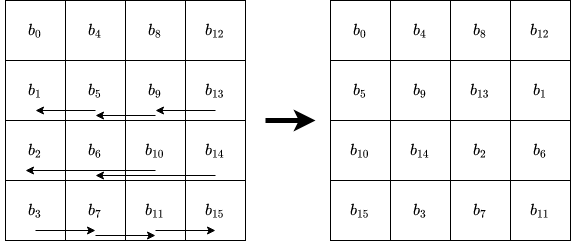
\includegraphics[width=.9\linewidth]{./Background/shiftRows.png}
\caption{\label{fig:ShiftRows}ShiftRows operation}
\end{figure}

MixColumns takes each column as a polynomial over the GF(2\textsuperscript{8}) and is multiplied (mod x\textsuperscript{4} +1,as it is a finite field) by \(a(x) = 3x^3 + x^2 + x + 2\), which can be written as a matrix as:
\[
\begin{bmatrix}
 s_{0,c}' \\
 s_{1,c}' \\
 s_{2,c}' \\
 s_{3,c}' \\
\end{bmatrix}=
\begin{bmatrix}
 2 & 3 & 1 & 1 \\
 1 & 2 & 3 & 1 \\
 1 & 1 & 2 & 3 \\
 3 & 1 & 1 & 2 \\
\end{bmatrix}
\begin{bmatrix}
 s_{0,c} \\
 s_{1,c} \\
 s_{2,c} \\
 s_{3,c} \\
\end{bmatrix}
\]
where c denotes the column multiplication is as described above and addittion is xor. By now the input text should be pretty diffused.

For decryption the equivalent inverse functions can be used, as Rijndahl is truely invertible, meaning an implementation in a reversible programming language would result in correct encryption or decryption based on whether the function was called or uncalled.

The original paper for Rijndahl\cite{Rijndahl} describes how these different steps can be implemented as using lookup tables. This implementation can be realised on any 32-bit system with 4096 bits of memory, as we would need 4 lookup tables of 256 32-bit entries. That is one table for each column with all the 256 values in GF(2\textsuperscript{8}). This approach are generally considered faster as it reduces each round to 16 lookups and 16 xors compared to the normal approach where memory needs to be moved around. As the decryption is truely invertible there exist likewise a lookup table approach for decryption.
\subsection{ChaCha20}
\label{ChaChaalg}
ChaCha20 is a stream cipher, which intend is to be a fast and efficient standby cipher in case AES is compromised. unlike block cyphers, such as AES, which works on a fixed sized block of text steam ciphers work on a per byte level. This is usually done by combining the plaintext with a pseudorandom stream of digits using XOR. As the objective of the cipher is to generate a random stream one first needs a seed. The seed of ChaCha is 16 32 bit words, layed out as such:
\begin{figure}[htbp]
\centering
\includegraphics[width=4cm]{./Background/ChaChaSeed.png}
\caption{\label{fig:ChaChaSeed}seed of ChaCha20}
\end{figure}

As one can see, the layout of the seed is fairly simple, and constitutes 4 parts:
\begin{itemize}
\item A 4 word constant ``expand 32-byte k'', which is a classic case of a ``nothing up my sleeve number''.
\item A 256 bit key in little endian order.
\item A word for the block counter (BC), which is sufficient for up to 256GB of plaintext.
\item A nonce which spans 3 word in little endian.
\end{itemize}
It might seem counter-intuitive that the seed would include a word, which holds the current block number. However the result of each iteration of chacha will result in 16 words generated for the stream. Since the rest of the seed will stay the same for the entire encryption the increasing block counter will ensure that no two ``blocks'' should result in the same cipher, and essentially including the CTR mode of operation for blockciphers into the streaming cipher. The confusion part of the algorithm follows a simple add-rotate-XOR (ARX) structure. That is every round is based on only simple arithmetic add, left rotations and XOR operations. more specifically ChaCha20 consist of 20 round of which each consists of 4 quarter rounds will confuse 4 input words. Each quarter round looks as such:
\begin{figure}[!htb]
\begin{minipage}{0.4\textwidth}
\begin{verbatim}
a += b; d ^= a; d <<<= 16;
c += d; b ^= c; b <<<= 12;
a += b; d ^= d; d <<<= 8;
c += d; b ^= c; b <<<= 7;
\end{verbatim}
\end{minipage}
\qquad
\begin{minipage}{0.4\textwidth}
\includegraphics[width=6cm]{Background/ChaChaQR.png}
\end{minipage}
\caption{ChaCha Quarter Round}
\label{fig:ChaChaQR}
\end{figure}
As said chacha20 will perform 20 round consisting of 4 quarter rounds. For the a quarter round in an even numbered round will take a column of the seed as the input. where an odd numbered round will work on diagonals.
\begin{figure}[!htb]
\centering
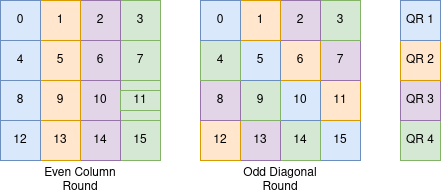
\includegraphics[width=8cm]{Background/diagonal.png}
\caption{ChaCha Rounds}
\label{fig:ChaChaRound}
\end{figure}
Lastly when the 20 rounds has been computed, the intial seed and the modifed version is index-wise added giving a resulting block of 16 words of stream and this stream can then be XORed with the plaintext to get the cypher.

\section{Implementation}
\label{sec:orgb7f8454}
\subsection{MD5}
\label{sec:orge427df0}

\subsubsection{naive}
\label{MD5naive}
As explained in section \ref{SME}, SME consists of busses and processes. We can define the MD5 algorithm naively using 4 busses and one simple process.


The compression function itself is completely contained in the single  clocked process and works as described in \ref{MD5alg}. The major difference comes in the data flow. Since our program will be mapped to hardware, we cannot have a variable sizes, everything has to be static. Thus we have opted for an approach which will receive 512 bits, corresponding to a single message block of the entire message, over the \texttt{Message} which we describe later. The process will both handle the padding and the compression and thus stand as a ``independent'' bus without depending on external computations.

For the bus-interface between the simulation process and the MD5 process we considered two overall approaches,
Firstly, one could have 2 inputbusses to the process, one which would contain the message and one which would contain the IV to modify. However, we find this approach unecessary as the initialisation vector is fixed for every hash. Thus the alternative. Since we use the c\# implementation of SME, we can easily store the Digest locally inside the process as a field. We will only require a single data bus with the message. we can define the Message bus as such:
\begin{verbatim}
    public interface IMessage : IBus {
        [InitialValue(false)] bool Valid { get; set; }

        [FixedArrayLength(MAX_BUFFER_SIZE)]
        IFixedArray<byte> Message { get; set; }

        int BufferSize { get; set; }
        int MessageSize { get; set; }

        [InitialValue(true)] bool Last { get; set; }
        [InitialValue(true)] bool Head { get; set; }
        [InitialValue(false)] bool Set { get; set; }
    }
\end{verbatim}
One can see there are multiple things to keep track of. First and foremost, all busses we will be working with should have a flag for whether or not a bus has data inside of it, since we try to adhere to the AXI protocol, which specifies some standards for a ready/valid handshake between the processes. Secondly, A byte-array is used to store the message block itself. \texttt{BufferSize} will be updated for every iteration or tick, and denotes how many values in the buffer are set, essentially flag for when the message should be padded. MessageSize will be set in the initial tick and denote the length of the entire message used for the Merkle-Damgård strengthening.
The last 3 flags are used to handle some ``edge-cases''.
Head Denotes that the initialization vector should be reconstructed.
Last is used to denote when a block is the last in the message. The block cannot be filled with more than 447 bits.
Set is used in the cases where the initial 1 should be set but where the block is not the last in the message, for instance when the length of the message is 448.

Since we also need to recive the digest from the process we also need an output bus. This bus is however fairly simple. It only consists of a Valid flag and the Hash as an array of 4 32-bit words.

Lastly we want 2 additional busses to make our design comply with the axi protocol. This bus will be the most basic of all busses and contain only a single flag, to show if the process is ready to receive data. It will thus be wired such that the MD5 process will have an ingoing bus to know when it is safe to send the digest to the simulation and an outgoing ready bus to let the simulation know when to send the message values.

\subsubsection{First optimization approach}
\label{sec:org1642614}
To make the algorithm more efficient, the length of the circuit produced in the VHDL code should be reduced. Meaning we want the simple process to do less. For the initial approach, we can notice that the compression function in MD5 works in rounds. Figure \ref{fig:MD5opt1} shows how the hash function as a whole up can be split up into 5 smaller processes and build a pipeline from this. One process for message formatting, and one for each of the 4 rounds. In our actual implementation we further added 2 processes:
\begin{itemize}
\item A message-converter process between the message formatting and \texttt{round 1 (f)} to convert the message from bytes to unsigned integers.
\item A combiner which does the last addition of the two vectors.
\end{itemize}

\begin{figure}[H]
\centering
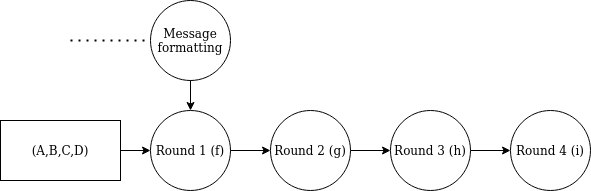
\includegraphics[width=.9\linewidth]{./Implementation/md5.png}
\caption{\label{fig:MD5opt1}MD5 pipeline}
\end{figure}
One problem we however have faced with this general approach is that MD5 is embarisingly sequential in the sense that \texttt{round 1 (f)} of the compression of the second message block 2, will depend of the result of \texttt{combiner} of the first message block's compression. This will create a stall. Thus for long messages the speed-up from the naive version should not be too considerable. However for very small messages (<448 bits) the throughput should be noticable faster as the propogation time should be decreased considerably. Hereby we expect to see a possibility to increase the clock frequency, which would tradeoff energy use for throughput.
\subsection{SHA256}
\label{sec:org1618b18}
SHA256 is a one way Secure Hash Algorithm. Which is where it gets its name from.
It is part of the SHA2 familiy and was designed and published by the NSA.
SHA256 is also build upon the Merkle-Damgård construction, like MD5.

The 256 part refers to the output size of 256-bit.
SHA256 can take in input of any size (depending on the implementation) but works
on chunks of 512-bits and then outputs a digest or hash of 256-bits.
Other versions from the SHA2 familiy exsits, like SHA512 and the truncated
versions like SHA224 and SHA384. If need should arise it would be simple to extend
the implementation of SHA256 to these other versions since it would mostly
consist of changing preset constants.

\subsubsection{naive}
\label{AESnaive}
\subsection{AES}
\label{sec:org812f731}

\subsubsection{naive}
\label{AESnaive}
Just like for the other algorithms AES can naively be implemented as a single simple process. That is we could implement the SME implentation of AES as a single process that can do both encryption and decryption and then have some checks in the \texttt{OnTick} function. This however poses some unwanted effects. First we add unecessary complication to the process as it would have to multiple things at once. Furthermore and more importantly a combined encrypter/decrypter reduces the utilizations of the library. Since AES is a block cypher and rarely only need to encrypt a block of 128 bits a sequence of blocks needs to be encrypted. This naive approach is not necessarily bad for some of the modes of operations such as Electronic Codebook (ECB) (which never really should be used anyway), Cipher Block chaining (CBC) (which eliminates parallelism) etc. as these will need a decryption algorithm. However is the programmer using this library choosing to operate under a Counter mode (CTR) or Galois-counter mode (GCM) the decryption algorithm itself would be unecessary as these modes uses the encryption function to both encrypt and decrypt. Thus in a hypotetical scenario where the design includes both encryption and decryption might take up 40 pct. of an FPGA and a design with only encryption would take up 20 pct. it is clear to see how many ressources is wasted. Thus we have decided that for the basecase implementation that encryption and decryption should be seperate processes. We will only go over the implementation of encryption as the process for decryption is the exact inverse computationally as described in section \ref{AESalg} and the structure thus follows symmetrically. For the design a single bus with 4 fields as seen below suffices. It consists of two Valid flags which works in a similar matter to the one described for MD5. Furthermore there is two byte arrays with the size of \texttt{BLOCK\_SIZE} = 128 as this implementation is a 128 bit key AES. We have one array for storing the data and one for storing the key. Once again we dont want to make the process itself flexible with multiple AES versions as reduces the resource utilization. If 128 key encryption suffices the overhead from including the 4 extra rounds for 256 is wasteful. Notice furthmore, the bus i named IPlainText but could just as well have been called IData or something similar as the same bus can be used for both the plaintext and the cypher as the algorithm is symmetrical.
\begin{verbatim}
    public interface IPlainText : IBus {
        [InitialValue(false)]
        bool ValidKey { get; set; }

        [FixedArrayLength(BLOCK_SIZE)]
        IFixedArray<byte> Key { get; set; }

        [InitialValue(false)]
        bool ValidData { get; set; }
        [FixedArrayLength(BLOCK_SIZE)]
        IFixedArray<byte> Data { get; set; }

    }
\end{verbatim}
For the actual process we follow the T-box approach described earlier, as we want the throughput of our FPGA to be as efficient as possible and comparable to fast CPU implementations, which of many has built in instructions that makes AES faster to compute such as, \texttt{GF2P8AFFINEINVQB}, \texttt{GF2P8AFFINEQB} and \texttt{GF2P8MULB}.
\subsubsection{optimisation 1}
\label{AESopt}
Just like for the other algorithms its is a quite slow approach to use only a single process and we can try to pipeline the different aspects of the algorithm as smaller processes, that is if we need the design to perform the encryption on multiple blocks. We notice that AES likewise uses rounds and each round can be divided into its own process. However we can note that each round does not have a lot of computation as we use the T-box implementation. The key-expansion might therefore be the most computationally heavy part and could be split into smaller parts, it is however worth noting that no matter the number of blocks to encrypt the key-expansion only needs to be calculated once, which also holds if we have multiple designs running in parallel on an FPGA.
\subsection{ChaCha}
\label{sec:org7ca66a2}

\subsubsection{naive}
\label{ChaChaNaive}
Just like the AES ChaCha will work in two phases. The initial phase will be to setup the the seed. After the initial setup, the only modification to the intial seed will be the block counter. We will thus have a similar bus to that of AES. The only difference is that we also need to give the nonce with the input bus. every iteration will perform chacha described in \ref{ChaChaAlg}. Just like for any of the other algorithms we have gone for a full solution, meanign the FPGA solution should be as independent as possible. This also means that our chacha20 version will not merely produce the stream but will produce the cipher itself.
\subsubsection{First optimization}
\label{ChaCha1}
As it should hopefully be clear from the high level description the computation of the rounds are quite simple compared to AES, which both needs computation in the key-expansion, and in the T-box version of AES a lot of table lookups. Furthermore ChaCha encourages concurrency and parallelism, as each ``block'' can be computed completely independently of each other. To start with we will however look at how the

\section{Results of implementation}
\label{sec:org281b80b}
All of the different implementations have been tested against the C\# standard library eqivalent algorithms and ensures that the results produced is correct. The only exception for this is Chacha as it is a quite uncommon cipher. All implementations synthesized using Xilinx Vivado, on a Zynq zedboard, which is a low-end FPGA. For comparisons we have chosen to include different implementations, in C, C\#, Cuda, and the openssl implemention. Unfortunately we have not been able to get our hands on the board in time and we thus stand with some limitations on the benchmarking results. Firstly, the reported frequency is the results from vivado, which might be a little different had it been an actual test.  Secondly, we settled for a raspberry pi 4B for the comparisons. The reason being this having a low-end processor similar to the one on the Zedboard, a Broadcom BCM2711, Quad core Cortex-A72 (ARM v8) 64-bit SoC @ 1.5GHz.
\subsection{MD5}
\label{sec:org0245a01}
MD5 naive: 2.38 Mhz
throughput: 512*2.38Mhz=1.218GBit=152,3MB/s
\subsection{SHA}
\label{sec:orgd1d4804}
SHA naive: 2.10 Mhz
throughput: 512*2.1Mhz=1.075GBit=134,4MB/s

\subsection{AES}
\label{sec:org9a84ce9}
AES naive: 25 Mhz
throughput: 128*25Mhz=3.2GBit=400MB/s

\subsection{CHACHA}
\label{sec:org7edb6f4}
ChaCha naive: ? Mhz
throughput: ?
fails nets before timing, too much data for a small board.

\section{Discussion}
\label{sec:org5b4590b}

\section{Conclusion}
\label{sec:orgb701c70}

\bibliographystyle{unsrt}
\bibliography{ref}

\begin{appendix}

\end{appendix}
\%\%\% Cha Cha er smart fordi den ikke bruger nogen ``advanceret'' operationer. Så specielle instruktioner på CPU'en kan ikke blive udnyttet
\%\%\% Så den burde virke lige så hurtig på hyper moderne optimeret CPU'er som på low power alternative CPU'er
\%\%\% Carl sagde vi kunne bruge: \url{https://www.ctan.org/pkg/ieeetran} til mødet
\%\%\% Nævn at både SHA256 og MD5 har samme opbygning.
\end{document}
